\newpage
\section{Appendix: Referenties}
\label{sec:app:Referenties}
  \subsection{Periodiek Systeem}  
  \label{sec:app:PeriodiekSysteem}
    
    \begin{rotate}{270}
	  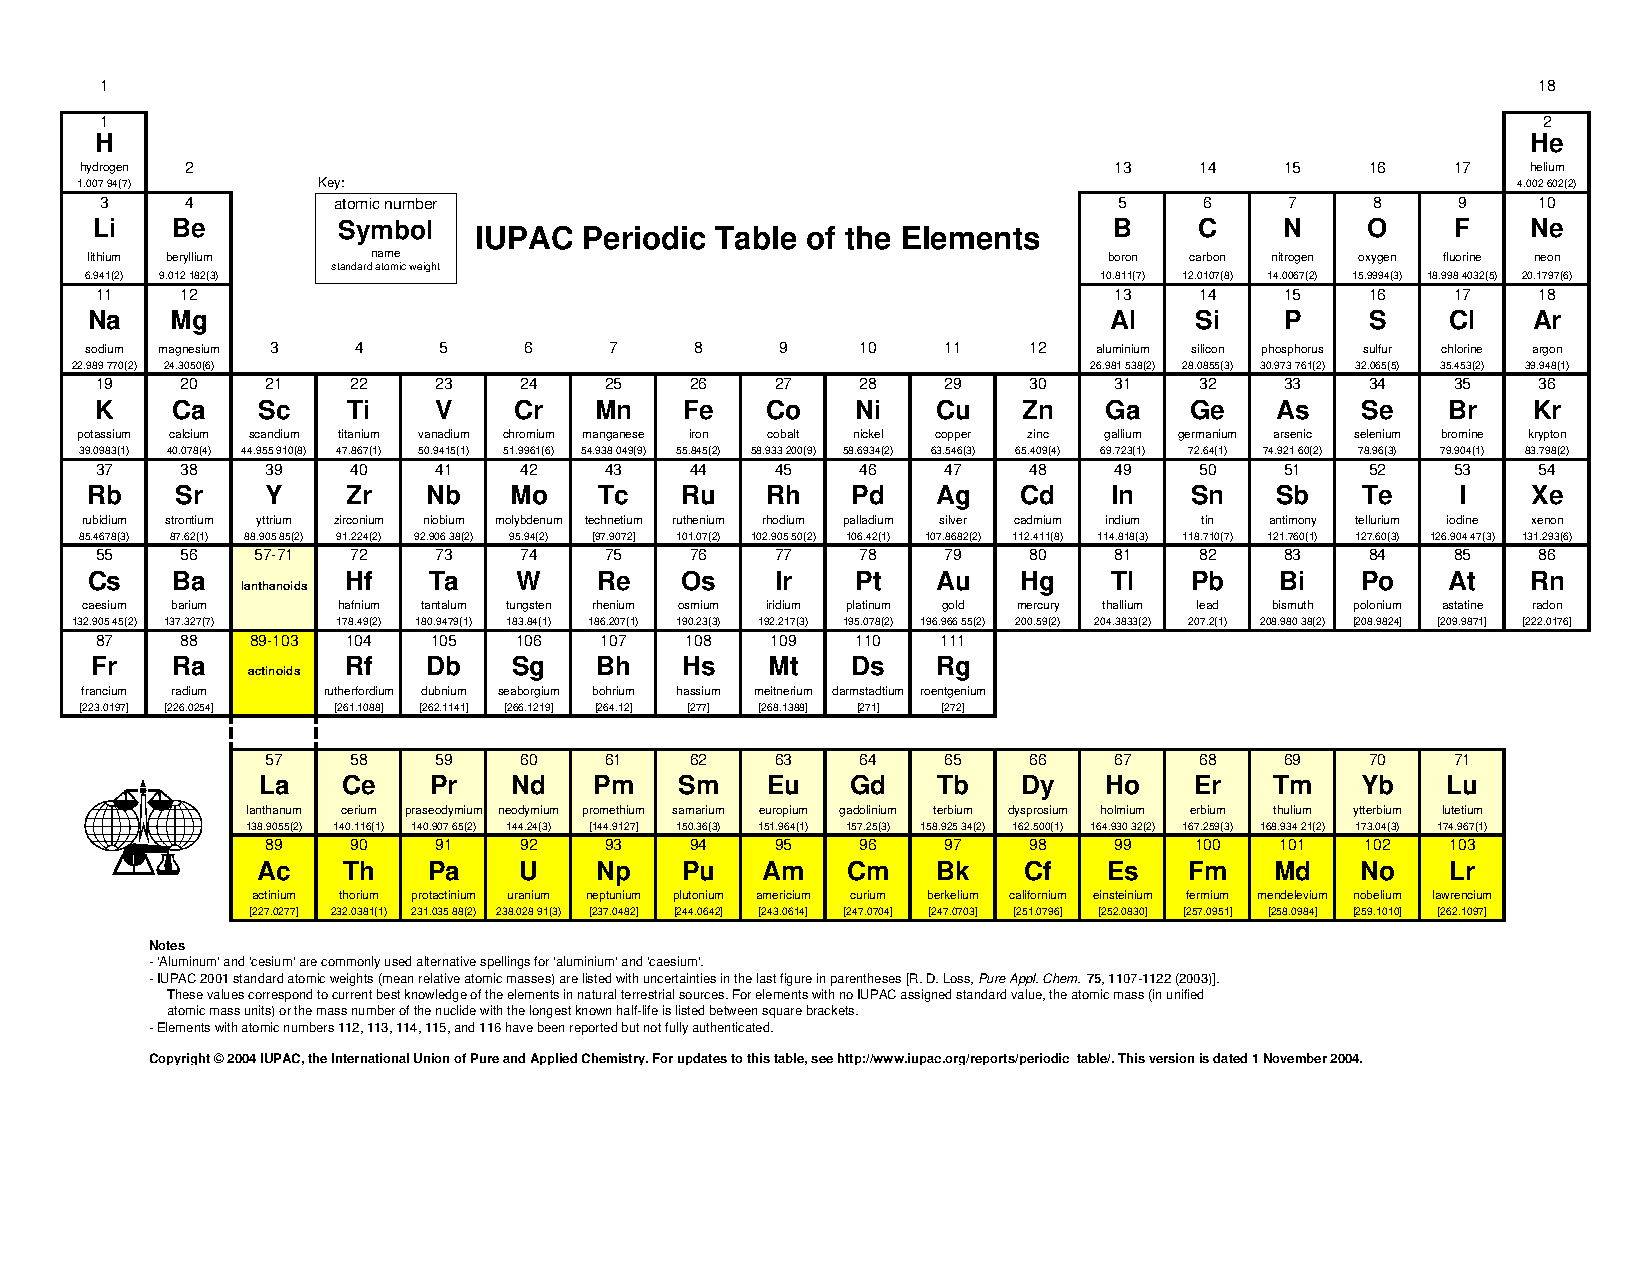
\includegraphics[width=1.00\textheight]{Appendix/PerSys.pdf}
    \end{rotate}
  \newpage
  
  \subsection{Fysische constanten}
  \label{sec:app:fysconstanten}
    \begin{tabular}{|l|c|r@{$,$}lll|}
      \hline
      \textbf{Naam} & \textbf{Symbool}  &  \multicolumn{3}{l}{\textbf{Waarde}}                   & \textbf{Eenheden}\\
      \hline
      Lading elektron        & $e$      & $1$ & $6021 $ & $ \cdot 10^{- 19}$   & $\eenh{C}$  \\ \hline
      Constante van Planck   & $h$      & $6$ & $6252 $ & $ \cdot 10^{- 34}$   & $\eenh{J}\eenh{s}$   \\ \hline
      Lichtsnelheid          & $c$      & $2$ & $99793$ & $ \cdot 10^{+ 08}$   & $\eenh{m}\eenh{s}^{-1}$ \\ \hline
      Massa van een elektron & $m_e$    & $9$ & $1083 $ & $ \cdot 10^{- 31}$   & $\eenh{kg}$  \\ \hline
      Massa van een proton   & $m_p$    & $1$ & $67239$ & $ \cdot 10^{- 27}$   & $\eenh{kg}$  \\ \hline
      Massa van een neutron  & $m_n$    & $1$ & $67470$ & $ \cdot 10^{- 27}$   & $\eenh{kg}$  \\ \hline
      Getal van Avogadro     & $N_A$    & $6$ & $0226 $ & $ \cdot 10^{+ 23}$   & $\eenh{mol}^{-1}$  \\ \hline
      Ideale gasconstante    & $R$      & $8$ & $314  $ &                      & $\eenh{J}\eenh{K}^{-1}\eenh{mol}^{-1}$ \\ 
                             &          & $0$ & $0820 $ &                      & $\eenh{l}\eenh{atm}\eenh{K}^{-1}\eenh{mol}^{-1}$ \\ 
                             &          & $1$ & $987  $ &                      & $\eenh{cal}\eenh{K}^{-1}\eenh{mol}^{-1}$ \\ \hline
      Constante van Blotzman & $\kappa$ & $1$ & $3805 $ & $ \cdot 10^{- 23}$   & $\eenh{J}\eenh{K}^{-1}$ \\ \hline
      Constante van Faraday  & $F$      & $96$ & $487 $ &                      & $\eenh{C}\eenh{mol}^{-1}$ \\ \hline
      Bohrstraal             & $a_0$    & $5$ & $2917 $ & $ \cdot 10^{- 27}$   & $\eenh{m}$  \\ \hline
      Valversnelling         & $g$      & $9$ & $81   $ &                      & $\eenh{m}\eenh{s}^{-2}$ \\ \hline
      \hline
      Correctiefactor 0001   & $\frac{RT}{F}\ln 10$       & $0$ & $0592 $ &    & \\ \hline
    \end{tabular}
  \subsection{Protolyseconstanten bij 25�C}
  \label{sec:app:protolyseconstanten}
    ..
  
  \subsection{Basiciteitsconstanten bij 25�C}
  \label{sec:app:basiciteitscontanten}
    ..
    
  \subsection{Standaardredoxpotentialen bij 25�C}
  \label{sec:app:redoxpotentialen}
    ..
    
  \subsection{Oplosbaarheidsproducten}
  \label{sec:app:oplosbaarheidsproducten}
    ..
    
  

  


